\documentclass[11pt,a4paper,titlepage]{article}
\usepackage[left=2cm,text={17cm,24cm},top=3cm]{geometry}
\usepackage[T1]{fontenc}
\usepackage[czech]{babel}
\usepackage[utf8]{inputenc}

\usepackage{graphicx}
\usepackage[ampersand]{easylist}
\usepackage{hyperref} % url
\bibliographystyle{czplain}

%uvozovky
\newcommand{\ceskeuvozovky}[1]{\quotedblbase#1\textquotedblleft}
\begin{document}

\begin{titlepage}
\begin{center}
    {\LARGE\textsc{Vysoké učení technické v~Brně}}\\
    \smallskip
    {\Large\textsc{Fakulta informačních technologií}}\\
    \bigskip
    \vspace{\stretch{0.382}}
    \Large{UPA - Ukládání a příprava dat}\\
    \smallskip
    \LARGE{Projekt: návrh zpracování a uložení dat}\\
    \smallskip
    \Huge{Téma: 04: COVID-19 (dr. Rychlý)}\\
    \vspace{\stretch{0.618}}
\end{center}
    {\Large Kapoun Petr, Bc. - xkapou04}\smallskip\\
    {\Large Nováček Pavel, Bc. - xnovac16}\smallskip\\
    {\Large Willaschek Tomáš, Bc. - xwilla00 \hfill \today }
\end{titlepage}

\tableofcontents
\newpage

% \part*{Projekt 1. část: návrh zpracování a uložení dat}
% \begin{center}
% Vysoké učení technické v~Brně\\
% Fakulta informačních technologií\\
% UPA - Ukládání a příprava dat\\
% \today
% \end{center}
\section{Zvolené téma}
04: COVID-19 (dr. Rychlý)
\section{Řešitelé}
\begin{itemize}
    \setlength\itemsep{0.3em}
    \item Bc. Kapoun Petr -- xkapou04,
    \item Bc. Nováček Pavel -- xnovac16,
    \item Bc. Willaschek Tomáš -- xwilla00.
\end{itemize}

\section{Zvolené dotazy a formulace vlastního dotazu}
\begin{itemize}
    \setlength\itemsep{0.3em}
    %\item dotaz A:
    \item \textbf{Dotaz A:} vytvořte popisné charakteristiky pro alespoň 4 údaje (např. věk, pohlaví, okres, zdroj nákazy) z datové sady COVID-19: Přehled osob s prokázanou nákazou dle hlášení krajských hygienických stanic (využijte krabicové grafy, histogramy, atd.).
    %\item v grafech zobrazte tempo změny počtů aktuálně nemocných (absolutní i procentuální přírůstek pozitivních případů a klouzavý průměr různých délek v různých časech)
    % \item dotaz B:
    %\item najděte skupiny nemocných s podobnými kritérii (např. podobný věk, místo, čas testů, atp.) a určete jejich vývoj v čase
    \item \textbf{Dotaz B:} určete vliv počtu nemocných a jeho změny v čase na sousední okresy (aneb zjistěte jak se šíří nákaza přes hranice okresů).
    %\item určete vliv epidemie COVID-19 na počet zemřelých v porovnání dle počtu nemocných, počtu hlášených úmrtí na nemoc COVID-19 a v porovnání s minulými lety
    %\item určete zpoždění změn přírůstku nemocných na přírůstek vyléčených v různých časech (aneb pokuste se odhadnout délku nemocnosti v různých časech)
    \item \textbf{Vlastní dotaz:} určete vliv věku na délku nemoci a úmrtnost.
    
\end{itemize}

\section{Stručná charakteristika zvolené datové sady}
% \textsc{Zde konkrétně popište jaké soubory budou představovat zdroj dat pro zvolené úlohy. Dále popište, jakým způsobem budou tato data získána a stručně charakterizujte strukturu souborů vybraných pro řešení projektu. Zaměřte se na části souborů, které jsou důležité pro zodpovězení zvolených dotazů.}

Základním zdrojem dat pro všechny dotazy jsou \textbf{otevřené datové sady COVID-19 v ČR}\cite{data_mzcr_covid_ofic} dostupné skrze veřejné API\footnote{\url{https://onemocneni-aktualne.mzcr.cz/api/v2/covid-19}} ve formátech JSON a CSV.

Datová sada \texttt{COVID-19: Přehled osob s prokázanou nákazou dle hlášení krajských hy\-gi\-e\-nic\-kých stanic (v2)} obsahuje následující charakteristiky o nakažených osobách:
\begin{itemize}
    \setlength\itemsep{0.3em}
    \item \texttt{datum} -- datum, kdy byla osoba pozitivně testována,
    \item \texttt{vek} -- věk nakažené osoby,
    \item \texttt{pohlavi} -- pohlaví nakažené osoby,
    \item \texttt{kraj\_nuts\_kod} -- identifikátor kraje podle klasifikace NUTS 3, ve kterém byla pozitivní nákaza hlášena krajskou hygienickou stanicí,
    \item \texttt{okres\_lau\_kod} -- identifikátor okresu podle klasifikace LAU 1,
    \item \texttt{nakaza\_v\_zahranici} -- příznak, zda došlo k nákaze mimo ČR,
    \item \texttt{nakaza\_zeme\_csu\_kod} -- identifikátor státu v zahraničí, kde došlo k nákaze (dvoumístný kód z číselníku zemí CZEM).
\end{itemize}

Další dvě použité datové sady jsou \texttt{COVID-19: Přehled vyléčených dle hlášení krajských hy\-gi\-e\-nických stanic} a \texttt{COVID-19: Přehled úmrtí dle hlášení krajských hygienických stanic}, které mají shodnou strukturu:
\begin{itemize}
    \setlength\itemsep{0.3em}
    \item \texttt{datum} -- datum vyléčení nebo úmrtí osoby,
    \item \texttt{vek},
    \item \texttt{pohlavi},
    \item \texttt{kraj\_nuts\_kod},
    \item \texttt{okres\_lau\_kod}.
\end{itemize}

Jelikož tyto datové sady používají identifikátory \textit{NUTS 3}\footnote{Nomenklatura územních statistických jednotek; úroveň 3 odpovídá krajům} pro kraje a \textit{LAU 1}\footnote{Local Administrative Units; úroveň 1 odpovídá okresům} pro okresy, využíváme dále číselníky od Českého statistického úřadu, které obsahují mapování těchto identifikátorů na odpovídající kraje a okresy a informace o nich.

\textbf{Číselník okresů}\footnote{Číselník okresů: \url{http://apl.czso.cz/iSMS/cisexp.jsp?kodcis=109&typdat=0&cisvaz=80007_210&datpohl=20.10.2020&cisjaz=203&format=2&separator=,}} a \textbf{číselník krajů}\footnote{Číselník krajů: \url{http://apl.czso.cz/iSMS/cisexp.jsp?kodcis=100&typdat=0&cisvaz=80007_885&datpohl=20.10.2020&cisjaz=203&format=2&separator=,}} jsou oba ve formátu CSV a obsahují:
\begin{itemize}
    \setlength\itemsep{0.3em}
    \item \texttt{KODJAZ} -- kód jazykové verze textů,
    \item \texttt{AKRCIS} -- akronym číselníku/klasifikace,
    \item \texttt{KODCIS} -- kód číselníku/klasifikace,
    \item \texttt{CHODNOTA} -- kód položky,
    \item \texttt{ZKRTEXT} -- zkrácený název položky,
    \item \texttt{TEXT} -- plný název položky,
    \item \texttt{ADMPLOD} -- počátek administrativní platnosti,
    \item \texttt{ADMNEPO} -- konec administrativní platnosti.
\end{itemize}

Zvoleným programovacím jazykem je \texttt{Python}\cite{python}. K získání dat použijeme standardní moduly jazyka \texttt{Python}\cite{python} 
\texttt{json}\footnote{Dokumentace modulu \texttt{json} jazyka \texttt{Python}\cite{python}: \url{https://docs.python.org/3/library/json.html}} a
\texttt{csv}\footnote{Dokumentace modulu \texttt{csv} jazyka \texttt{Python}\cite{python}: \url{https://docs.python.org/3/library/csv.html}}. K nahrání dat použijeme modul \texttt{elasticsearch}\footnote{Modul \texttt{elasticsearch} pro \texttt{Python}: \url{https://pypi.org/project/elasticsearch/}}.

\section{Zvolený způsob uložení uložení surových dat}
% \textsc{Zde stručně charakterizujte NoSQL databázi, která bude využita pro uložení zvolených zdrojových dat.}

Pro uložení dat jsme zvolili NoSQL řešení \texttt{Elasticsearch}\cite{elastic}\footnote{Dokumentace \texttt{Elasticsearch}\cite{elastic}: \url{https://www.elastic.co/guide/en/elasticsearch/reference/current/index.html}}. \texttt{Elasticsearch} je dokumentově orientovaný vyhledávací engine naprogramovaný v jazyce Java s použitím \texttt{Lucene}\cite{lucene}, díky kterému je velmi efektivní při komplexním vyhledávání na velkých objemech dat. Schéma struktur kolekcí odpovídá struktuře uložených dat ve vstupních datových sadách. Index je typu klíč-hodnota a pro každý vstupní soubor bude existovat právě jeden index. Klíč nabývá hodnoty \texttt{CHODNOTA} u číselníku okresů a krajů a ve zbývajících indexech se generuje automaticky, protože data neobsahují žádnou unikátní hodnotu.

\newpage
\section{Implementace}
Výsledné řešení obsahuje skripty pro:
\begin{itemize}
    \item nahrání dat do \texttt{NoSQL} databáze,
    \item doplnění, spojení a transformace dat z \texttt{NoSQL} do \texttt{SQL},
    \item prezentaci výsledku ve webovém rozhraní. 
\end{itemize}
Dále obsahuje \texttt{Docker}\cite{docker} kontejner, ve kterém jsou nainstalované aplikace databází.

Výsledné řešení neobsahuje inkrementální aktualizaci dat, protože mechanismus pro tuto aktualizaci by jednak byl pomalejší než přeplnění a jednak to není ani možné.
Pomalejší by byl z toho důvodu, že datová sada ve formátu \texttt{CSV} není vytvořená jako inkrementální, ale data jsou vložena náhodně. Pro inkrementální doplnění dat do \texttt{NoSQL} databáze (například po měsících) by bylo potřeba načíst celý soubor, seřadit jej a následně plnit rozdílné měsíce/dny (přičemž plnění do \texttt{Elasticsearch} je velmi rychlé).

Inkrementální transformace těchto dat do \texttt{SQL} není následně možná z důvodu aplikace heuristiky, která mapuje jednotlivé případy vyléčení a úmrtí k záznamu nákazy. Tuto inkrementální aktualizace znemožňuje fakt, že data jsou do datových souborů přidávána i zpětně, tedy když je osoba označena za vyléčenou a za pár dní přibude podobný případ vyléčení, není jisté, s jakou osobou se má spojit.


\subsection{Předání vstupních dat}
Pro nahrání dat určených ke zpracování a vyhodnocení aplikací slouží webová stránka, která akceptuje pouze oficiální datové formáty (\texttt{json}, \texttt{CSV}). Vstupní soubor lze také specifikovat pomocí \texttt{URL}. Tento mechanismus zjednodušuje práci se skripty a umožňuje spustit celou aktualizaci z UI. 

Mechanismus dále validuje vstupní data a upozorňuje na chyby (například neznámý formát) a zobrazuje stav plnění v konzoli.

Díky tomu, že je implementace plnění dat poměrně obecná, bylo by možné nahrát data například z jiného státu a zobrazit si pro něj výsledky.


% Očekávaný formát

% \begin{verbatim}
%     ALLOWED_CODES = {
%     'states': ['CHODNOTA', 'ZKRTEXT'],
%     'regions': ['CHODNOTA1', 'TEXT1'],
%     'neighbours': ['HODNOTA1', 'HODNOTA2'],
%     'infected': ['datum', 'vek', 'pohlavi', 'kraj_nuts_kod', 'okres_lau_kod', 'nakaza_v_zahranici', 'nakaza_zeme_csu_kod'],
%     'recovered': ['datum', 'vek', 'pohlavi', 'okres_lau_kod'],
%     'dead': ['datum', 'vek', 'pohlavi', 'okres_lau_kod']}
% \end{verbatim}

% Díky tomu, že je to implementováno vcelku genericky, by bylo např. možné nahrát soubory pro jiný stát, a nechat si udělat statistiky pro něj (tj. teoreticky se nefixujeme jen na výchozí datové sady od našeho statistického úřadu; prakticky - vykreslujeme mapu čr u druhého dotazu:D )

% po spuštění aplikace je potřeba nejprve skrze tuto stránku data nahrát, aplikace nepustí uživatele nikam dál
% Po validaci dat dojde k jejich importování; během toho lze vidět průběh v "konzoli"; při importu nelze provádět další činnosti (ani nový import, ani nic)

% Po importu se zobrazí výsledky všech dotazů. byl implementován  filtr podle měsíců. Data a stránka s výsledky jsou perzistentní, dokud se uživatel nerozhodne pro nahrání nových dat, pak je zde funkce na vymazání všeho a import nových dat



\subsection{Rozšíření datové sady}
Pro druhý dotaz byla potřeba informace o sousednosti okresů. Pro tento účel vznikl další soubor ve formátu \texttt{CSV}. Obsahuje dva názvu okresů, které spolu sousedí:
\begin{itemize}
    \setlength\itemsep{0.3em}
    \item \texttt{HODNOTA1} -- název okresu,
    \item \texttt{HODNOTA2} -- název okresu.
\end{itemize}

\subsection{NoSQL databáze}
Do \texttt{NoSQL} databáze \texttt{Elasticsearch} jsou nahrány všechny záznamy ze vstupních souborů za použití funkcí knihovny \texttt{Pandas} (v případě \texttt{CSV} souborů), nebo načtení a vložení vstupního souboru \texttt{JSON}. 

\newpage
\subsection{SQL databáze}
Vytvořená \texttt{SQL} databáze má následující schéma:
\newline \newline
\begin{figure}[h]
    \centering
    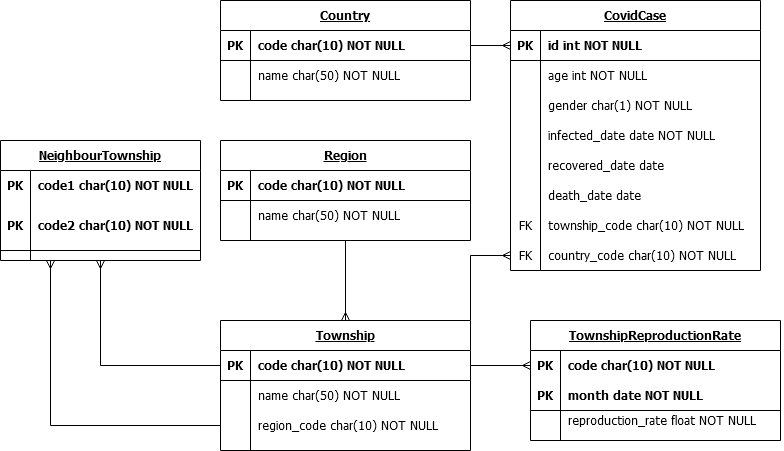
\includegraphics[width=0.70\textwidth]{img/sql_schema.png}
    \label{fig:}
\end{figure}
\\
\textbf{Postup plnění:}
\begin{enumerate}
    \item vytvoření \texttt{SQL} databáze podle definovaného modelu,
    \item vyčítání dat z \texttt{Elasticsearch},
    \item aplikování heuristiky pro propojení případů vyléčení/úmrtí se záznamem onemocnění,
    \item uložení dat do \texttt{MySQL}.
\end{enumerate}
\\
\textbf{Heuristika pro spojení záznamů:}
\begin{enumerate}
    \item Iteruj přes všechny okresy.
    \setlength{\itemindent}{1em}
    \item Vezmi všechny záznamy nakažených pro aktuální okres a seřaď je vzestupně podle data nakažení.
    \item Vezmi všechny záznamy uzdravených pro aktuální okres z \texttt{NoSQL} databáze a seřaď je vzestupně podle data uzdravení.
    \item Vezmi všechny záznamy zemřelých pro aktuální okres z \texttt{NoSQL} databáze a seřaď je podle data úmrtí.
    \item Iteruj přes všechny získané záznamy nakažených.
    \setlength{\itemindent}{2em}
    \item Pro aktuální záznam nakaženého najdi první odpovídající záznamy (tj. záznamy se stejným věkem a pohlavím) v záznamech uzdravených a zemřelých, pro které platí, že jejich datum uzdravení/úmrtí je mladší, než datum nakažení aktuálního záznamu.
    \item Pokud jsou nalezeny záznamy pro obě skupiny, pak:
    \setlength{\itemindent}{3em}
    \item Aktuálnímu záznamu nakaženého přiřaď to datum, které je z nalezených záznamů uzdravení/úmrtí starší, použitý záznam odstraň a pokračuj.
     \setlength{\itemindent}{2em}
    \item Pokud je nalezen pouze jeden záznam, pak:
     \setlength{\itemindent}{3em}
        \item Přiřaď jeho hodnotu data aktuálnímu záznamu nakaženého, odstraň ho a pokračuj.
    \setlength{\itemindent}{2em}
    \item Jinak pokračuj dalším záznamem nakaženého.
    \setlength{\itemindent}{0em}
\end{enumerate}
    
\newpage
\section{Prezentace výsledků}
Pro prezentaci výsledků byl použit framework \texttt{Flask}\footnote{Dokumentace modulu \texttt{Flask} jazyka \texttt{Python}\cite{python}: \url{https://pypi.org/project/Flask/}}, který umožňuje zobrazeni vytvořených výsledků jednoduše ve webovém rozhraní.
Výsledky za celé období nahraných dat jsou perzistentní, lze je aktualizovat až nahráním nových dat. Webové rozhraní dále umožňuje si zobrazit statistiky za konkrétní období, avšak toto chvíli trvá, protože databáze obsahuje mnoho záznamů.

\subsection{Dotaz A}
\begin{quote}
Vytvořte popisné charakteristiky pro alespoň 4 údaje (např. věk, pohlaví, okres, zdroj nákazy) z datové sady COVID-19: Přehled osob s prokázanou nákazou dle hlášení krajských hygienických stanic (využijte krabicové grafy, histogramy, atd.).
\end{quote}

Vytvořili jsme popisné charakteristiky a jejich vývoj v čase pro následující údaje:
\begin{itemize}
    \item věk,
    \item pohlaví,
    \item nákaza,
    \item úmrtí,
    \item zdroj nákazy.
\end{itemize}

\newpage
\subsubsection{Kumulativní nárůst případů}
Jde o vyplněný spojnicový graf, který zobrazuje celkový kumulativní počet případů v čase.
\begin{figure}[h]
    \centering
    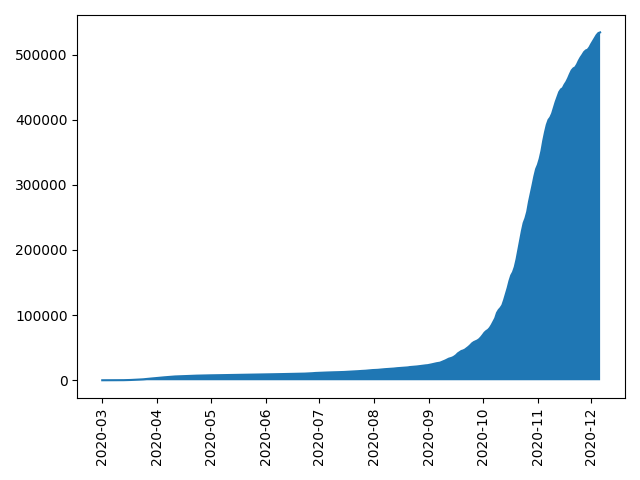
\includegraphics[width=0.70\textwidth]{img/cumulative_cases.png}
    \label{fig:cumulative_cases}
\end{figure}

\subsubsection{Kumulativní nárůst úmrtí}
Jde o vyplněný spojnicový graf, který zobrazuje celkový kumulativní počet případů v čase.
\begin{figure}[h]
    \centering
    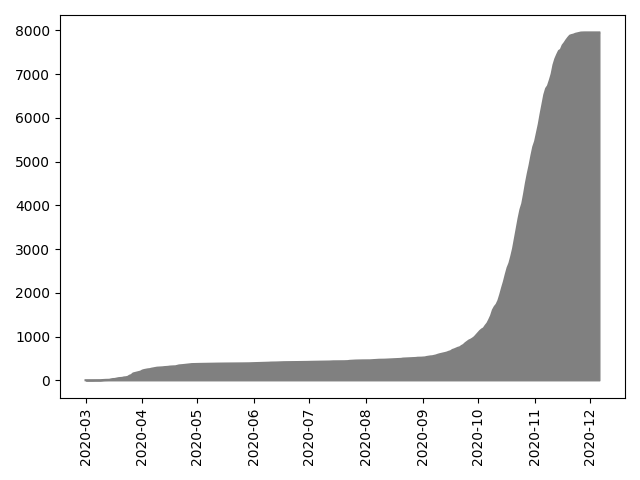
\includegraphics[width=0.70\textwidth]{img/cumulative_deaths.png}
    \label{fig:cumulative_deaths}
\end{figure}

\newpage
\subsubsection{Denní přírůstek podle věkových skupin}
Jedná se o spojnicový graf, kde každá spojnice reprezentuje denní přírůstek pro určitou věkovou skupinu. Tento graf je doporučeno zobrazit si na webu pro určité období, protože data jsou čitelnější.
\begin{figure}[h]
    \centering
    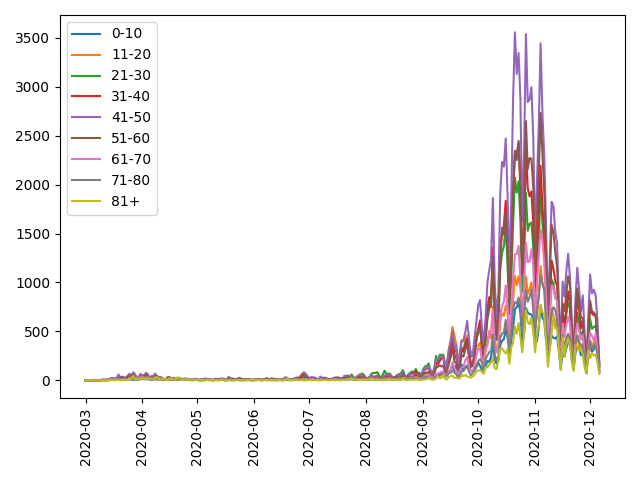
\includegraphics[width=0.70\textwidth]{img/increase_by_age.png}
    \label{fig:daily_by_age}
\end{figure}

\subsubsection{Úmrtnost podle věkových skupin}
Jedná se o pruhový graf, který zobrazuje celkový počet obětí, pro danou věkovou skupinu v čase.
\begin{figure}[h]
    \centering
    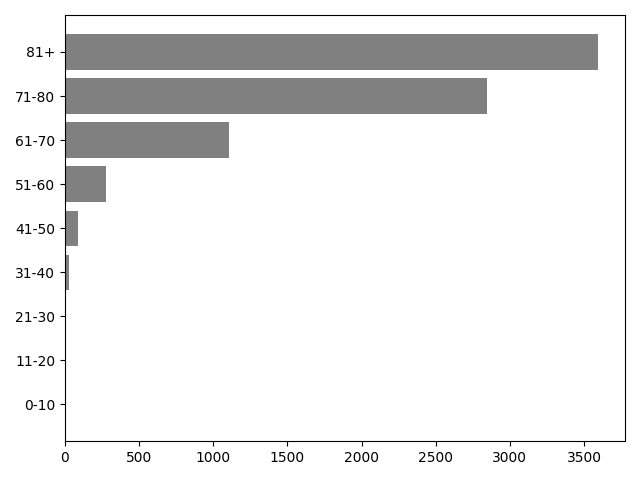
\includegraphics[width=0.70\textwidth]{img/mortality_by_age.png}
    \label{fig:mortality_by_age}
\end{figure}

\newpage
\subsubsection{Úmrtnost podle pohlaví}
Jde o spojnicový graf, kde každá ze spojnic reprezentuje denní úmrtnost podle pohlaví v čase.
\begin{figure}[h]
    \centering
    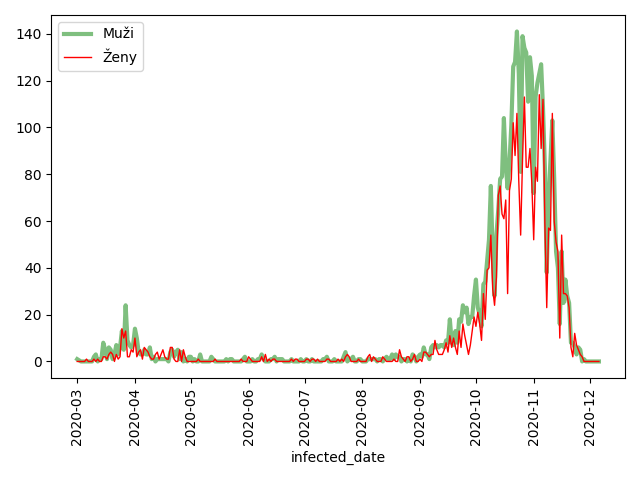
\includegraphics[width=0.65\textwidth]{img/mortality_by_sex.png}
    \label{fig:mortality_by_sex}
\end{figure}

\subsubsection{Původ nákazy (pro více než 10 případů)}
Jedná se o bodový graf, kde jednotlivé body reprezentují zdroj nákazy českých občanů v zahraničí. Graf pro přehlednost zobrazuje jen státy, kde se v konkrétním dni nakazilo více než 10 osob.
\begin{figure}[h]
    \centering
    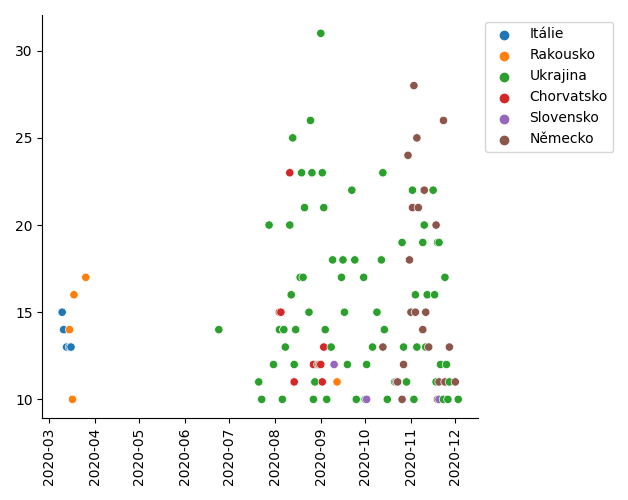
\includegraphics[width=0.70\textwidth]{img/external_country.png}
    \label{fig:external_country}
\end{figure}

\newpage
\subsection{Dotaz B}
\begin{quote}
Určete vliv počtu nemocných a jeho změny v čase na sousední okresy (aneb zjistěte jak se šíří nákaza přes hranice okresů).
\end{quote}
Dotaz klade důraz na změny v čase, proto zodpovězení dotazu vychází z výpočtu reprodukčního čísla, které vyjadřuje v dotazu právě onu změnu v čase. Výpočet čísla je zjednodušený a jde v podstatě o procentuální změnu přírůstku nakažených.

\subsubsection{Orientovaný graf}\label{dotazb_ograf}
Při znázornění velikosti reprodukčního čísla a vztahu okresů jsme nejdříve použili nástroj graphviz a jeho modul pro \testtt{Python}\cite{python}. Hodnoty použité pro vytvořený orientovaný graf byly použity při tvorbě mapy popsané v \ref{dotazb_mapa}. Uzly v grafu znázorňují okresy. Barva uzlů znázorňuje velikost reprodukčního čísla. Hrana vyjadřuje sousednost okresů. Orientace hran grafu je určena porovnáním velikostí reprodukčních čísel dvou okresů. Hrana vychází z uzlu okresu, který má větší hodnotu reprodukčního čísla.
\begin{figure}[h]
    \centering
    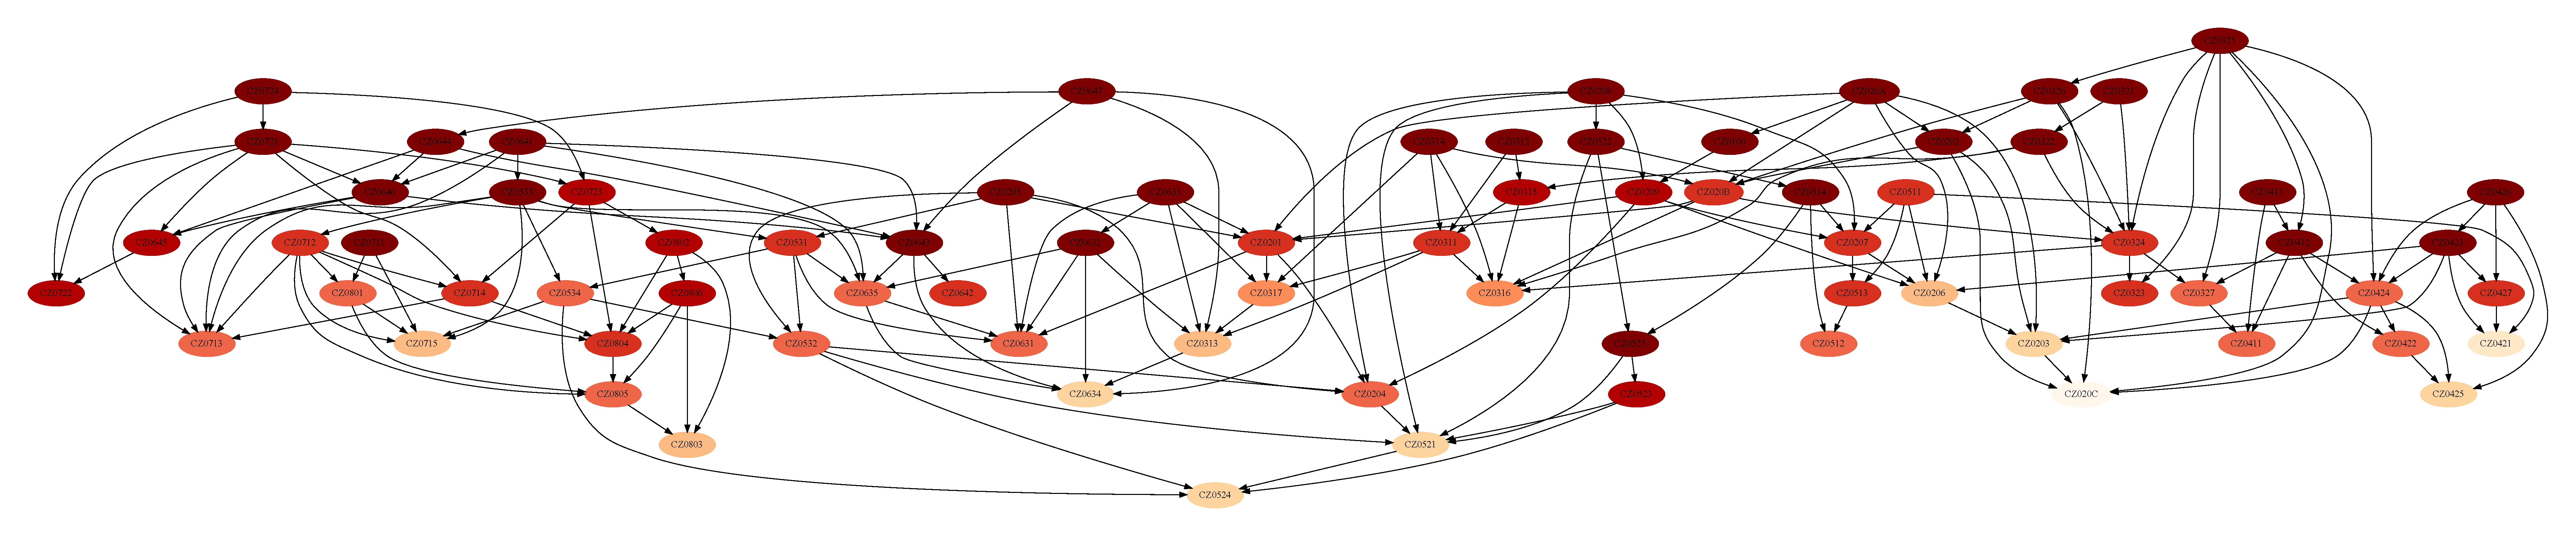
\includegraphics[width=\textwidth]{img/fsm.gv.pdf}
    \label{fig:external_country}
\end{figure}

\subsubsection{Mapa}\label{dotazb_mapa}
Pro znázornění velikosti reprodukčního čísla a vztahu okresů byla vytvořena mapa, která podobně jako orientovaný graf popsaný v \ref{dotazb_ograf}, nastavuje barvu okresu podle reprodukčního čísla. Malé červené trojúhelníky znázorňují šíření nákazy z více nakažených okresů do méně nakažených okresů. Postup nákazy je zobrazen orientací trojúhelníku.

\begin{figure}[h]
    \centering
    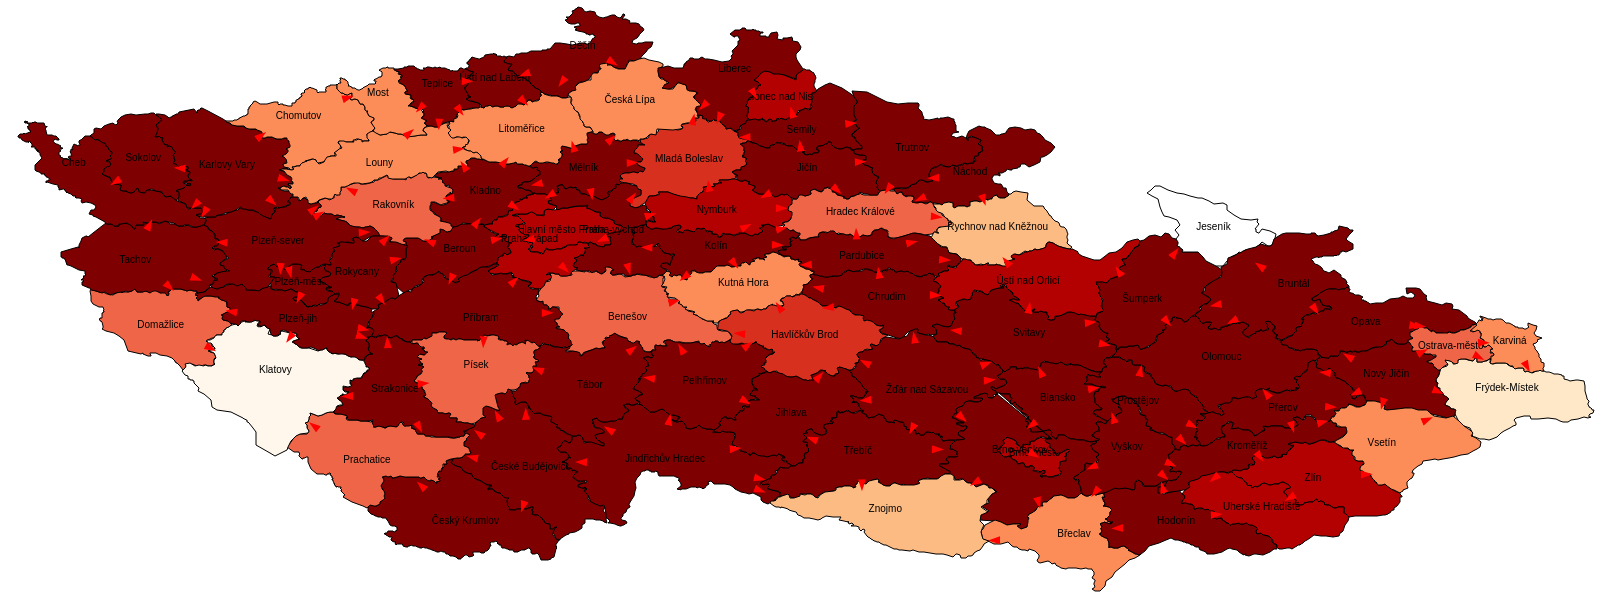
\includegraphics[width=\textwidth]{img/mapa.png}
    \label{fig:external_country}
\end{figure}
\newpage
\subsubsection{Graf průměrného reprodukčního čísla sousedních okresů vzhledem k reprodukčnímu číslu okresu}
Jde o bodový graf, kde pro každý okres je vykreslen jeden bod. Souřadnice \texttt{X} vyjadřuje reprodukční číslo okresu. Souřadnice \texttt{Y} vyjadřuje průměrné reprodukční číslo okolních okresů.

Z grafu je patrné mírné stoupání hodnot v závislosti na hodnotě osy \texttt{X}. Přehledněji vliv sousedních okresů ukazují grafy zobrazené v \ref{dotazb_graf1}
\begin{figure}[h]
    \centering
    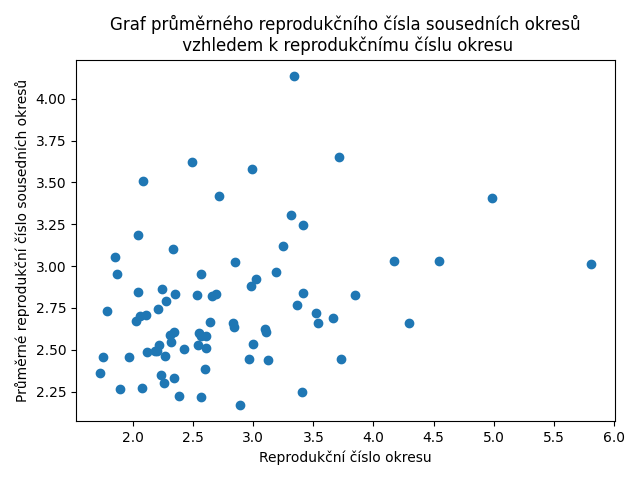
\includegraphics[width=0.70\textwidth]{img/graf_okresy02.png}
    \label{fig:external_country}
\end{figure}

\newpage
\subsubsection{Grafy průměrného rozdílu reprodukčních čísel sousedních okresů k reprodukčnímu číslu okresu a průměrného rozdílu reprodukčních čísel všech okresů k reprodukčnímu číslo okresu}\label{dotazb_graf1}
Jde o bodové grafy, kde pro každý okres jsou vykresleny dva body:
\begin{itemize}
    \item \textbf{Oranžové kruhy} - průměrný rozdíl reprodukčních čísel sousedních okresů vzhledem k reprodukčnímu číslu okresu
    \item \textbf{Modré trojúhelníky} - průměrný rozdíl reprodukčních čísel všech okresů vzhledem k reprodukčnímu číslo okresu
\end{itemize}
Souřadnice \texttt{Y} vyjadřuje průměrný rozdíl reprodukčního čísla vůči reprodukčnímu číslu daného okresu. Tyto dva grafy se liší významem souřadnice \texttt{X}. Souřadnice X prvním grafu vyjadřuje pořadové číslo okresu po seřazení okresů dle velikosti reprodukčního čísla a v druhém grafu vyjadřuje reprodukční číslo okresu. Graf s osou \texttt{X} znázorňující reprodukční číslo přesněji zobrazuje data, ale protože je okres relativně malé území, tak při menší časové jednotce může při výpočtu vyjít velmi vysoká hodnota (10-12) reprodukčního čísla, při které je naprostá většina hodnot koncentrována na malé ploše, což má za následek nepřehlednost grafu. To je důvod pro vytvoření dvou grafů.

Z grafů je patrné, že rozdíly se sousedními okresy jsou menší než rozdíly se všemi okresy. Takový jev potvrzuje vliv sousedních okresů na nákazu v okrese.

\begin{figure}[h]
    \centering
    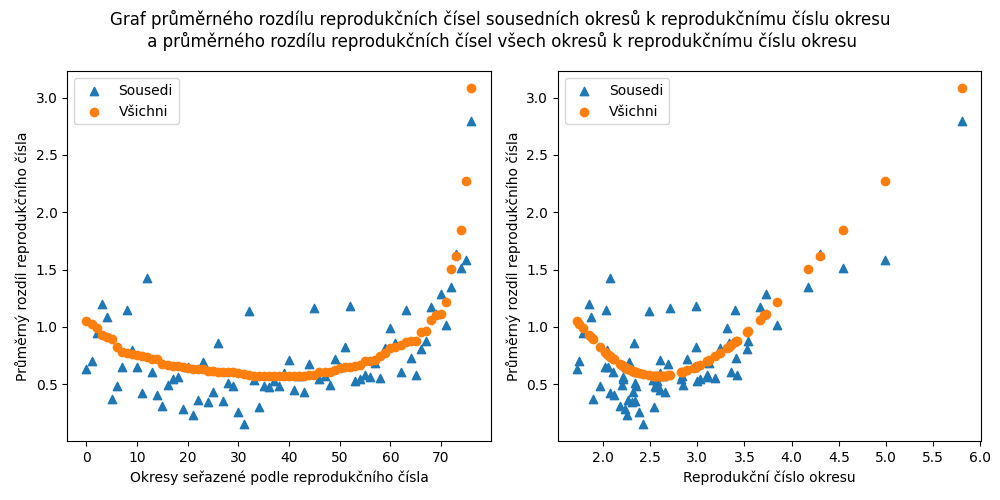
\includegraphics[width=\textwidth]{img/graf_okresy01.png}
    \label{fig:external_country}
\end{figure}

\newpage
\subsection{Vlastní dotaz}
\begin{quote}
Určete vliv věku na délku nemoci a úmrtnost.
\end{quote}

\begin{figure}[h]
    \centering
    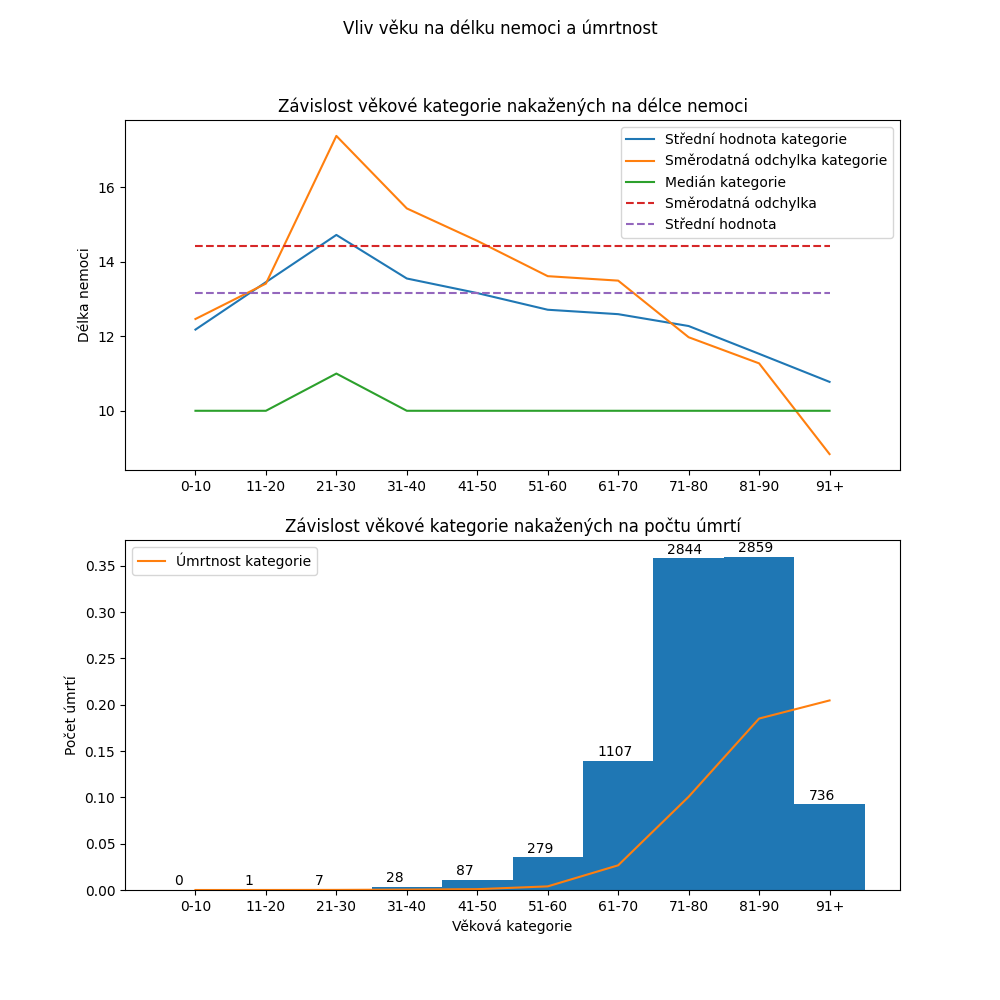
\includegraphics[width=\textwidth]{img/vlastni_dotaz.png}
    \label{fig:external_country}
\end{figure}

\newpage
\section{Návod k použití}
Projekt využívá \texttt{Docker}\cite{docker} a jazyk \texttt{Python}\cite{python}. K zajištění závislostí lze spustit:
\begin{quote}
    \verb|./setup.sh|
\end{quote}
Následující příkaz připraví a spustí docker image:
\begin{quote}
    \verb|./run.sh -b -esr -sqlr|
\end{quote}
Aplikaci je možné spustit ve dvěma způsoby.
Spuštění webové aplikace, kterou lze otevřít v prohlížeči na adrese \textit{localhost}:
\begin{quote}
    \verb|python run.py --web|
\end{quote}
Spuštění přes příkazovou řádku:
\begin{quote}
    \verb|python run.py --fill|\\
    \verb|python run.py --move|\\
    \verb|python run.py --queries|
\end{quote}



% \url{https://blog.kuzzle.io/what-nosql-solution-should-you-choose-mongodb-elastisearch-oriendb}



\newpage
\bibliography{literatura}

\end{document}

% \subsection{Kumulativní a denní přehledy dle KHS a laboratoří}
% 1. COVID-19: Celkový (kumulativní) počet provedených testů (v2) - \textsc{testy.(json/csv)}
% \begin{itemize}
%     \item datum
%     \item prirustkovy\_pocet\_testu
%     \item kumulativni\_pocet\_testu
% \end{itemize}

% 2. COVID-19: Celkový (kumulativní) počet osob s prokázanou nákazou dle krajských hygienických stanic včetně laboratoří (v2) - \textsc{nakaza.(json/csv)}
% \begin{itemize}
%     \item datum
%     \item prirustkovy\_pocet\_nakazenych
%     \item kumulativni\_pocet\_nakazenych
% \end{itemize}

% 3. COVID-19: Celkový (kumulativní) počet osob s prokázanou nákazou dle krajských hygienických stanic včetně laboratoří, počet vyléčených, počet úmrtí a provedených testů (v2) - \textsc{nakazeni-vyleceni-umrti-testy.(json/csv)}
% \begin{itemize}
%     \item datum
%     \item kumulativni\_pocet\_nakazenych
%     \item kumulativni\_pocet\_vylecenych
%     \item kumulativni\_pocet\_umrti
%     \item kumulativni\_pocet\_testu
% \end{itemize}

% 4. COVID-19: Základní přehled - \textsc{zakladni-prehled.(json/csv)}
% \begin{itemize}
%     \item datum
%     \item provedene\_testy\_celkem
%     \item potvrzene\_pripady\_celkem
%     \item aktivni\_pripady
%     \item vyleceni
%     \item umrti
%     \item aktualne\_hospitalizovani
%     \item provedene\_testy\_vcerejsi\_den
%     \item potvrzene\_pripady\_vcerejsi\_den
%     \item potvrzene\_pripady\_dnesni\_den
% \end{itemize}

% \subsection{Přehledy dle KHS}
% 5. COVID-19: Přehled osob s prokázanou nákazou dle hlášení krajských hygienických stanic (v2) - \textsc{osoby.(json/csv)}
% \begin{itemize}
%     \item datum
%     \item vek
%     \item pohlavi
%     \item kraj\_nuts\_kod
%     \item okres\_lau\_kod
%     \item nakaza\_v\_zahranici
%     \item nakaza\_zeme\_csu\_kod
% \end{itemize}

% 6. COVID-19: Přehled epidemiologické situace dle hlášení krajských hygienických stanic podle okresu - \textsc{kraj-okres-nakazeni-vyleceni-umrti.(json/csv)}
% \begin{itemize}
%     \item datum
%     \item kraj\_nuts\_kod
%     \item okres\_lau\_kod
%     \item kumulativni\_pocet\_nakazenych
%     \item kumulativni\_pocet\_vylecenych
%     \item kumulativni\_pocet\_umrti
% \end{itemize}

% 7. COVID-19: Přehled vyléčených dle hlášení krajských hygienických stanic - \textsc{vyleceni.(json/csv)}
% \begin{itemize}
%     \item datum
%     \item vek
%     \item pohlavi
%     \item kraj\_nuts\_kod
%     \item okres\_lau\_kod
% \end{itemize}

% 8. COVID-19: Přehled úmrtí dle hlášení krajských hygienických stanic - \textsc{umrti.(json/csv)}
% \begin{itemize}
%     \item datum
%     \item vek
%     \item pohlavi
%     \item kraj\_nuts\_kod
%     \item okres\_lau\_kod
% \end{itemize}
